%!TEX root = ../template.tex
%Developed using Sublime Text 3 with LaTexTools plugin
%SUPER+b for compiling latex to pdf
%Don't forget to use SUPER+R to jump between top level commands!
%%%%%%%%%%%%%%%%%%%%%%%%%%%%%%%%%%%%%%%%%%%%%%%%%%%%%%%%%%%%%%%%%%%%
%% chapter2.tex
%% UNL thesis document file
%%
%% Chapter with the template manual
%%%%%%%%%%%%%%%%%%%%%%%%%%%%%%%%%%%%%%%%%%%%%%%%%%%%%%%%%%%%%%%%%%%%
\chapter{State of the Art}
\label{cha:state_of_the_art}
% ================
% = Introduction =
% ================

The most common methods used in the detection of turn insulation faults in \acrshort{ims} are those based on models and intelligent systems. As for model-based, the most conventionally used set of techniques are the \acrfull{esa}, while intelligent systems are presented in various 
procedures.

\acrshort{esa} is the general term for a set of electrical machine condition monitoring techniques through the analysis of electrical signals such as current and voltage. Several works report the use of those techniques applied to turn insulation fault detection, presented in section \ref{sec:conventional_techniques}. However, one issue that is rarely discussed is the need for rapid response to prevent catastrophic damage when an interturn short-circuit fault arises. This topic is addressed in section \ref{subsec:resolution_fast_response}.

The use of intelligent systems have gain a lot of momentum and are target of recent works, where the most related to this dissertation's goal  are presented in section \ref{sec:machine_learning_approaches}.



\section{Conventional Techniques for fault detection} % (fold)
\label{sec:conventional_techniques}

Analyse the current and voltage of several components of the motor and instantaneous power to detect problems is common practice ~\cite{Bonaldi2012}. These kind of analysis  are aim to detect problems such as faults in the stator, rotor problems, problems on the engagement, efficiency problems, among others. These kind of analysis supposes that the motor electrical and mechanical internals can be thought of as a transfer function  that converts the input voltage waveform into the output current waveform (figure \ref{fig:motor_transducer}), allowing electrical signals (voltage and/or current) to carry information of the electrical and mechanical problems.
These analysis are not something easy to be done, because it involves a set of comparisons with previously stored patterns and own "history" of the motor being analyzed ~\cite{Bonaldi2012}. 


\subsection{Symmetrical components: Negative Sequence and Zero sequence } % (fold)
\label{subsec:negative_sequence_current_compensation}

Symmetrical components is a technique used to simplify the analysis of an unbalanced \acrshort{tp} machine. The idea is that an asymmetrical set of $N$ phasors can be expressed as a linear combination of $N$ symmetrical set of phasors by means of a complex linear transformation. The resulting $N$ symetrical phasors can be referred to as positive, negative or zero.

A positive sequence (or direct sequence) is a set of phasors that are equal in magnitude and lag 120º in a clock-wise direction. In figure \ref{fig:positive_negative_sequence}, it can be seen a positive voltage sequence. 

A negative sequence (or inverse sequence) is a set of phasors that are equal in magnitude and lag 120º in a counter clock-wise direction. In figure \ref{fig:positive_negative_sequence}, it can be seen a negative voltage sequence. 

A zero sequence (or homopolar sequence)  is a set of phasors that are equal in magnitude but are not lagged. Since there is no rotation sequence due to not existing delay, this is called a zero sequence.

\begin{figure}[htbp]
\centering
 \subbottom[Positive sequence components]{%
    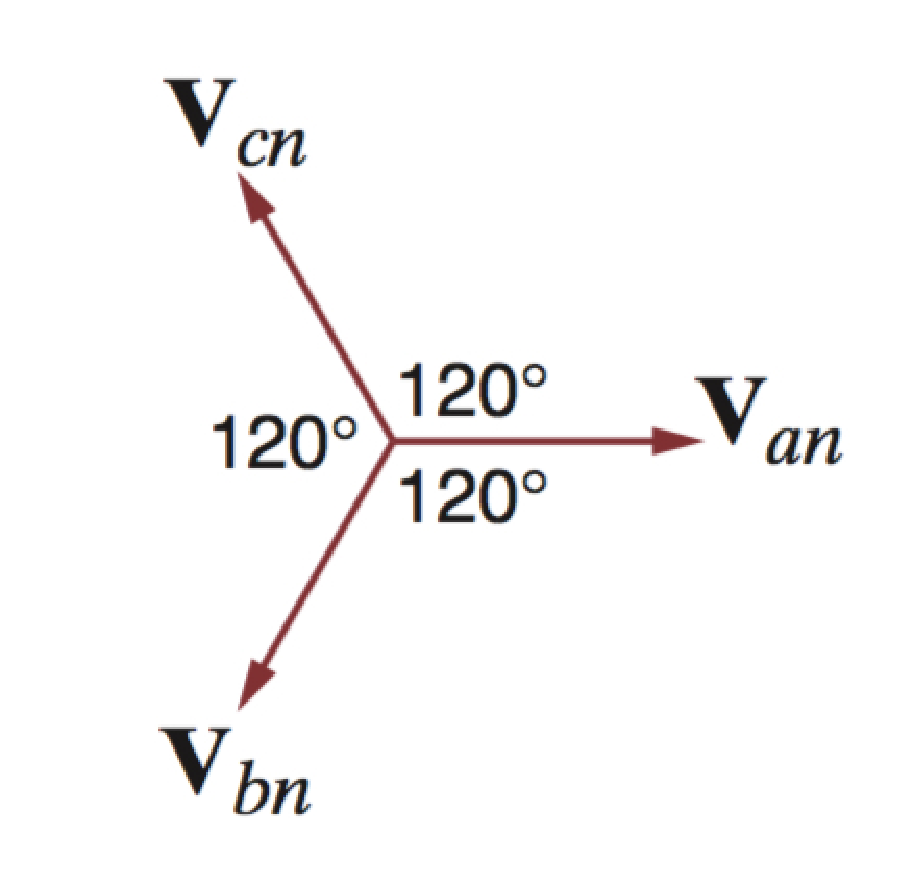
\includegraphics[width=0.4\linewidth]{phasorDiagramExample}}%
 \subbottom[Negative sequence components]{%
    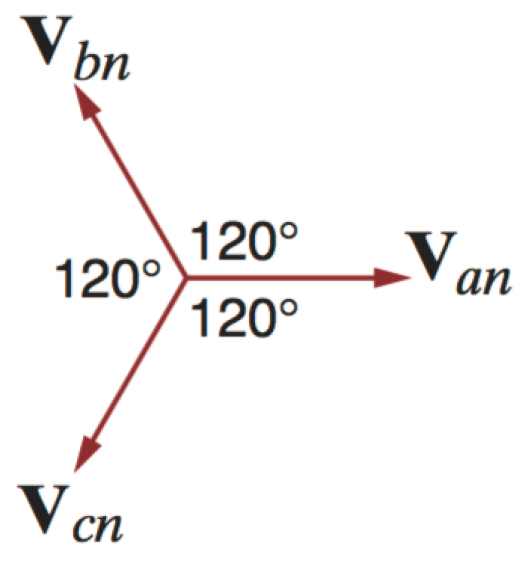
\includegraphics[width=0.3\linewidth]{negativesequence.png}}
\caption{Positive sequence components and Negative sequence components }
\label{fig:positive_negative_sequence}
\end{figure}

\todo[inline]{fazer a alteração da imagem da componente negativa como pdf, e fazer a edição no photoshop as a pdf}


When an interturn short-circuit fault arises, another physical phenomenon that enables the fault detection is the appearance of a negative-sequence component in the supply currents ~\cite{Cabanas2013}. The faulty phase has fewer turns than the healthy phases, generating less electromotive force and having difference impedance, which leads to an unbalanced system of three-phase currents

In ~\cite{Bouzid2013}, it's deduced an analytical expression for the symmetrical components of the steady-state stator phase current under several windings faults, such as interturn short-cirtuit and phase-to-phase short-circuit. From this study, the author has shown that the phase angle of the negative sequence current is a robust indicator of stator fault and is able to effectively locate the faulty phases, since it is insensitive neither to the load conditions nor to the voltage unbalance and the frequency variation ~\cite{Bouzid2013}. Further, the author also suggests that zero sequence current is useful to detect the phase-to-ground fault and discriminate between interturn short-circuit and phase-to-ground short-circuit.


Still, these methods have an handicap: other causes not related to short-circuit faults can also introduce a negative-sequence component in the current (unbalanced supply voltage, constructive asymmetries), reducing the sensitivity of early faults detection. Regarding this handicap, in ~\cite{Bakhri2012} the authors introduce a technique for the compensation of negative-sequence current components that are not related to stator faults, including the effect of voltage unbalance, allowing to detect even small stator shorted turn faults.  



\subsection{Machine Current Signature Analysis} % (fold)
\label{subsec:mcsa}
\acrfull{mcsa} is a technique based on the monitoring of the input current of the motor, and it's used to analyze and monitor the trend of dynamic energized systems.By monitoring the stator currents it is possible for the user to analyze the produced current spectrum, referred as motor signature. This provides insights on the motors, by identifying the magnitude and frequency of each individual component that integrates the motor current signal, without the need to stop the motor. The diagnostic is typically done by comparing the spectrum of the monitored current with the expected spectrum of the motor if it was in an healthy state.

\begin{figure}[htpb]
\centering
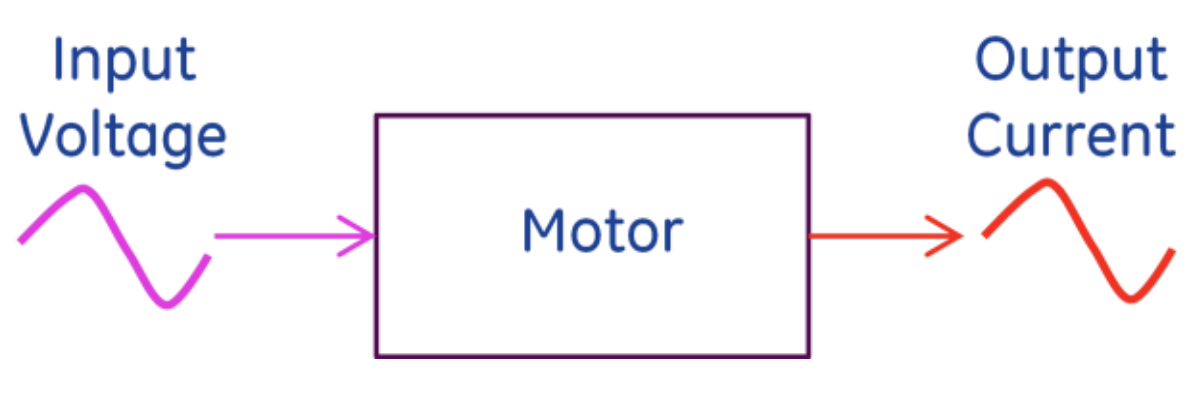
\includegraphics[width=0.5\textwidth]{motor_as_a_function.png}
\caption{Motor as a function, where the input is the voltage and the output is the current}
\label{fig:motor_transducer}
\end{figure}

The motor current signature is recorded in a time domain format, resulting in a wave form as shown in figure \ref{fig:three_phase_sampled}.

\begin{figure}[htpb]
\centering
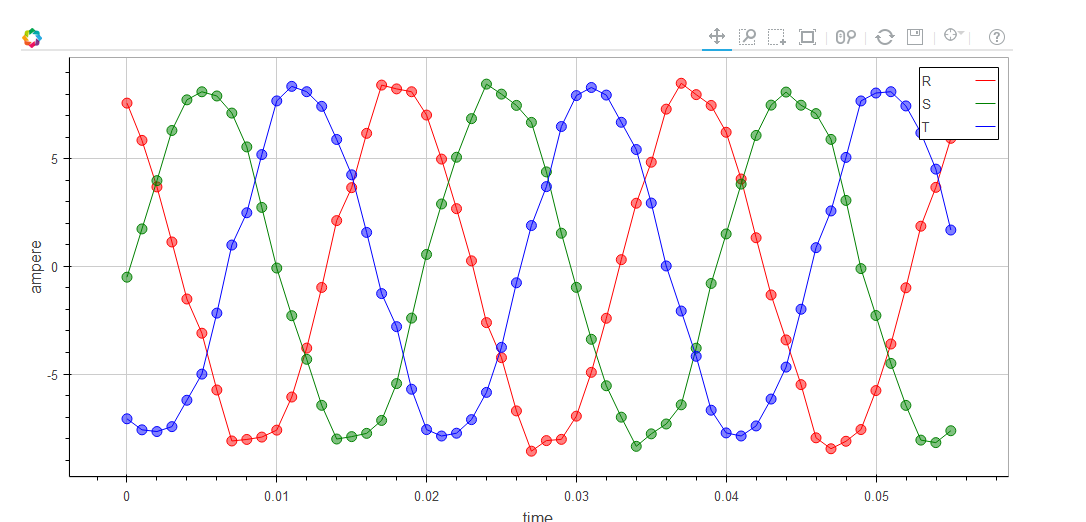
\includegraphics[width=0.9\textwidth]{three_phase_waveform.png}
\caption{Sampled three phase currents of a motor}
\label{fig:three_phase_sampled}
\end{figure}

In order to analyse the power spectrum the main tool employed is the \acrfull{fft} ~\cite{Bonaldi2012}, in spite of some systems employ in conjunction with other techniques to increase the ability of fault detection from signal acquisition, through processing, up to the diagnosis step. An example of a \acrshort{fft} output's plot can be seen in figure \ref{fig:frequency_fft}.


\begin{figure}[htpb]
\centering
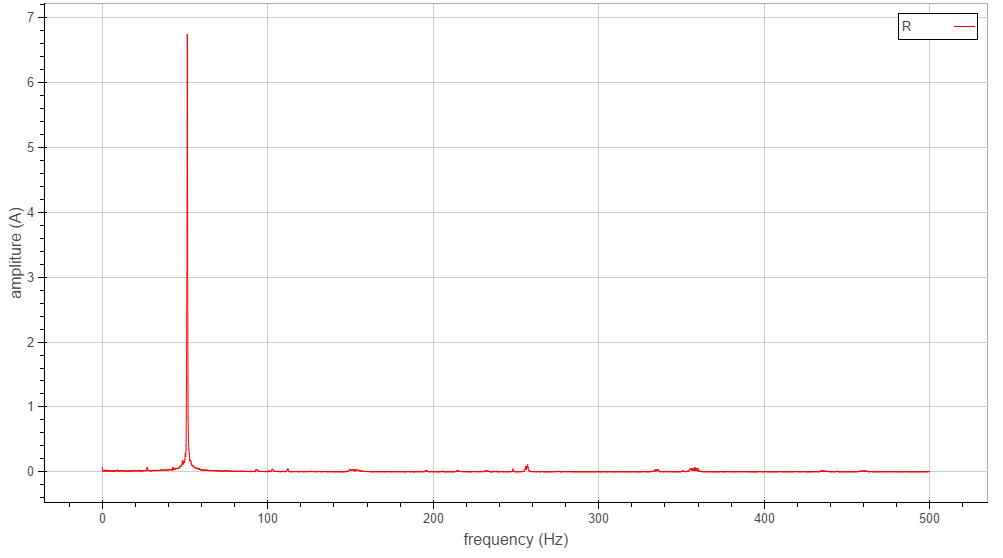
\includegraphics[width=0.7\textwidth]{frequency_fft.png}
\caption{Current Spectrum of an healthy motor sampled at 1kHz}
\label{fig:frequency_fft}
\end{figure}


\acrshort{fft} is an algorithm that computes the \acrfull{dft}. The \acrshort{fft} computes the transform in $O(n\log{}n)$, which has lower time complexity than the \acrfull{dft}, which has a time complexity of $O(n^2)$.

Concerning the  \acrshort{fft}, it is important to approach the Nyquist theorem. This theorem states that for any signal to be reconstructed without significant losses, the sample frequency must be twice of the maximum frequency presented on the signal. For example, if the objective is to analyse frequencies on a signal up to 500 Hz, the sample frequency must be 1kHz.

In ~\cite{Penman1994} the authors detected stator winding interturn short-circuits patterns by analysing the axial leakage flux components of the current using a flux sensor. 
Axial flux is the horizontal magnetic flux (parallel to the shaft) generated by the stator. For the ideal machine the axial leakage flux is zero, but in practice asymmetries exist due to imperfections in winding geometry as well as non-uniformities present in the materials of construction ~\cite{Penman1994}. They formulated a mathematical model for the frequency components of inter-turn short circuited, which depends on the values of motor slip, number of poles, power supply frequency and rotor angular speed. Since these kind of failures don't reproduce new frequencies in the current spectrum,  ~\cite{Penman1994} states that it could be difficult to detect stator faults through current spectrum only using \acrshort{mcsa}. 

Although, in ~\cite{Jung2006} the author have demonstrated, through a lot of experimental results on \acrshort{ims}, that interturn short-circuit can be detected accurately in stator windings of low voltage \acrshort{ims} by using \acrshort{mcsa}, mathematical formulas and a digital signal processing techniques for high-speed signal processing and advanced signal-and-data-processing.


\subsection{Park's Vector and Extended Park's Vector Approach} % (fold)
\label{subsec:epva}

The Park's Vector analysis consists in the transformation of the stator currents into Park's vector, through the equation \ref{eq:parks_vector}.

\begin{equation} \label{eq:parks_vector}
    \begin{cases}
	    i_{d}(t) =  \sqrt[2]{\frac{2}{3}} i_A(t) - \sqrt[2]{\frac{1}{6}} i_B(t) - \sqrt[2]{\frac{1}{6}} i_C(t) \\
	    i_{d}(t) =  \sqrt[2]{\frac{1}{2}} i_B(t) - \sqrt[2]{\frac{1}{2}} i_C(t) 
	\end{cases}
\end{equation}

 Under ideal conditions, the Park's Vector has the following components:
\begin{equation} \label{eq:parks_vector_d_ideal_cond}
    i_D = (\frac{\sqrt{6}}{2})i_M sin(\omega t)
\end{equation}
\begin{equation} \label{eq:parks_vector_q_ideal_cond}
    i_D = (\frac{\sqrt{6}}{2})i_M sin(\omega t - \frac{\pi}{2})
\end{equation}
 
\noindent where
    $i_M$ is the maximum value of the current positive sequence (A),
    $\omega$ is the angular supply frequency (rad/s),
    and $t$ is the time variable (s)

The corresponding representation is a perfect circle, as shown in figure \ref{fig:park_vector_circle} (a).
Although, under fault conditions, equations \ref{eq:parks_vector_d_ideal_cond} and \ref{eq:parks_vector_q_ideal_cond} are not valid. since the motor supply current will contain other components besides the positive-sequence component, leading to a representation as shown in figure \ref{fig:park_vector_circle} (b).

\begin{figure}[htbp]
\centering
 \subbottom[Park's vector of an healthy motor]{%
    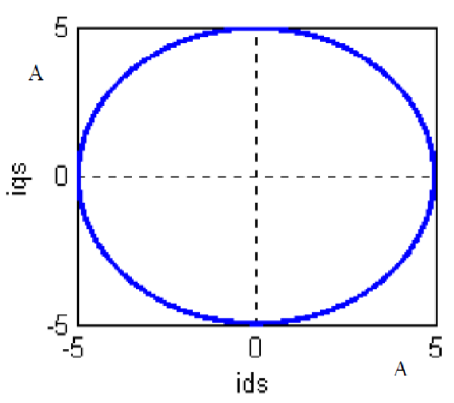
\includegraphics[height=0.3\linewidth]{park_healthy_motor.png}}%
 \subbottom[Park's vector of an damaged motor]{%
    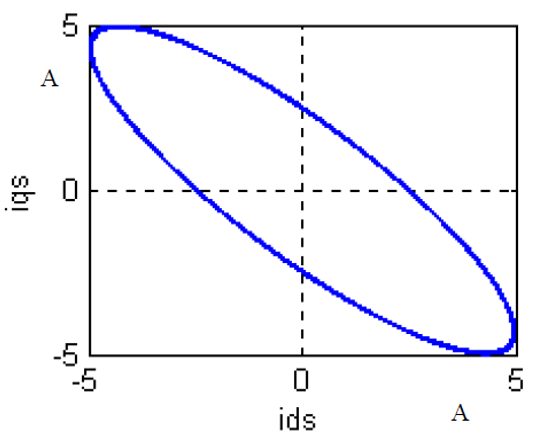
\includegraphics[height=0.3\linewidth]{park_damaged_motor.png}}
\caption{Positive sequence components and Negative sequence components }
\label{fig:park_vector_circle}
\end{figure}
 
 
 The \acrfull{epva} is a simple and efficient diagnosis method based on the spectral analysis of Park's vector modulus (PVM) which is computed as:
 
\begin{equation} \label{eq:parks_vector_modulus}
    PVM = \sqrt{(i_d^2 + i_q^2)}
\end{equation}

By taking into account the current in all the three phases, this method provides a more meaningfull spectrum than the one obtained by the conventional motor current spectral analysis.
 
This techniques was used to detect stator winding faults in operating \acrshort{tp} motors in  ~\cite{Cruz2001}, where it shows the ability of the EPVA to detect stator circuit faults, even when these are strictly confined to the degradation of the stator magnetic circuit.

%%%%%%%%%%%% Park-Hilbert Method %%%%%%%%%%%%
\subsection{Park-Hilbert Method} % (fold)
\label{subsec:park_hilbert_method}

This method starts by applying the \acrfull{ht} to the three phase currents, resulting in an analytical signal. From this analytical signal, the extended park's vector analysis is computed, resulting in the Park's vector modulus. At this point, a new generated signal arises called \acrfull{pvmph}.
This method is based on spectral analysis, by applying the \acrshort{fft} to the \acrshort{pvmph} signal.

The \acrshort{ht} is a signal analysis method frequently used in diverse scientific fields. Mathematically, the \acrshort{ht} of a real signal $x(t)$ (like the phase current) can be defined as the time domain convolution of $x(t)$ with $\frac{1}{t}$ and can accentuate the local properties of the real signal as follows:

\begin{equation} \label{eq:convolution_signal_ht}
    y(t) = HT{x(t)} = \frac{1}{\pi t} \ast x(t) = \frac{1}{\pi} \int_{- \infty}^{\infty} \frac{x(\tau)}{\tau - t} d \tau 
\end{equation}

The analytical signal $ \bar{x}(t) $ is obtained by coupling $x(t)$ with its \acrshort{ht} as follows;

\begin{equation} \label{eq:analytical_function}
    \bar{x}(t) = x(t) + jy(t) = a(t)e^{j\theta (t)}
\end{equation}

\noindent with

\begin{equation} \label{eq:analytical_function_a}
    a(t) = \sqrt{2}{ [ x^2(t) + y^2(t) ]}
\end{equation}

\begin{equation} \label{eq:analytical_function_o}
    \theta(t) = arctan\left (\frac{x(t)}{y(t)} \right)
\end{equation}

where $a(t)$ is the instantaneous amplitude of the $\bar{x}(t)$, and $\theta(t)$ is the instantaneous phase of the $\bar{x}(t)$.

With this transformation, it is possible to study the changes that happen on both amplitude and phase (independently) of any signal acquired from the machine.

In ~\cite{Kia2013}, the authors state that this techniques allows to suppress the fundamental frequency component and to work only with failure frequencies, making it easier to the fault detection process. In the same work, it is also state that this technique  sensitive to winding faults. Compared with \acrshort{mcsa} and \acrshort{epva}, ~\cite{Kia2013} proves that the \acrshort{pvmph} is more sensitive to the occurrence of an incipient shorted turns.

\subsection{Resolution and Fast Response} % (fold)
\label{subsec:resolution_fast_response}

One issue that is rarely discussed is the need for a rapid response to prevent a catastrophic damage when an interturn short-circuit fault happens. For example, if the conventional fast Fourier transform (FFT) is used to detect faulty components in an early stage, an high-frequency resolution is required. This leads to long sampling periods, which could be longer than the time needed to prevent a catastrophic failure when the fault arises. 

As stated in ~\cite{Cheng2011}, an analysis on the trade off between resolution and fast response is needed. The authors of ~\cite{Cheng2011} use a sampling time of 0.25 seconds, which leads to a frequency resolution of 4Hz, for calculating the spectrum of the complex current vector to detect positive and negative sequence currents.

In this context, effective approaches need to use signal-processing techniques for achieving appropriate frequency resolution with short sampling periods. They should as well not have heavy computational complexities, so that processing almost in real time may be accomplishable ~\cite{Riera-Guasp2015}. 

\section{Intelligent Systems for fault detection} % (fold)
\label{sec:machine_learning_approaches}
Artificial Intelligence techniques can be used to classify the state of the motor into a series of classes, like healthy state, different types of faulty states and different fault severity degree whithout the need of complex mathematical formulas ~\cite{Riera-Guasp2015}. In ~\cite{Gandhi2011} it is concluded that artificial models provide a fast and accurate simulation of the machine once they are trained.
However, these models are motor specific and require extensive training to provide good results under all conditions.

\subsection{Artificial Neural Networks} % (fold)
\label{sec:ann}


\Acrfullpl{ann} are classifiers inspired by Biology. As all kind of classifiers, an \Acrshort{ann} goal is to maximize the likelihood for the predicted result of a given input to be as close as possible of the real result. This goal is accomplished by training the \Acrshort{ann} , which will adapt the consideration of the input against the expected result of that input. This classifier provides a general method for learning functions from examples, being the examples real-valued, discrete-valued, or vector-valued.

\Acrshort{ann} are composed by perceptrons, which are units that take a vector of real-valued inputs, calculates a linear combination of these inputs, and then computes a function which will give the result, as seen in figure \ref{fig:sigmoid_unit}.

\begin{figure}[htpb]
\centering
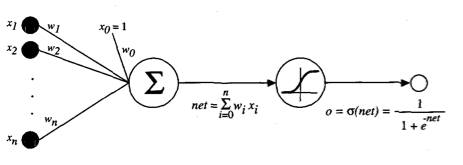
\includegraphics[width=0.5\textwidth]{sigmoidunit.png}
\caption{A perception unit with sigmoid activation function}
\label{fig:sigmoid_unit}
\end{figure}

Each perceptron have a linear combination so that a value may be produced from the input vector. from figure \ref{fig:sigmoid_unit}, it can be seen that each input has its own weight. So, for example, a simple linear combination could be such as the equation \ref{eq:linear_combination}.

\begin{equation} 
\label{eq:linear_combination}
\sum_{i=1}^{n} w_{i}*x_{i}
\end{equation}

For example, if the \Acrshort{ann} is composed by only one perceptron, after it computes the linear combination, this value is applied to a function which will give us the class. For example, in a binary classification problem, the activation function can be the Logistic Function - also called sigmoid function.

In ~\cite{Jawadekar2014}, the authors present a multiple faults detection system for an induction motor based on an \Acrshort{ann} (three-layer feedforward neural network). For signal processing, they use the \acrfull{cwt} since it can be effective in analyzing stationary (steady-state) and non stationary (transient) signals under a non-sinusoidal supply condition.

In this context, the use of the \acrshort{cwt} is appropriate since it gives information about the signal in the domains of frequency and time.
Mathematically, the \acrshort{cwt} of a real signal $x(t)$ is defined as follows:

\begin{equation} 
\label{eq:wavelet_transform}
    W_f(a,b) = \int_{- \infty}^{\infty}  x(t) \psi_{ab}^*(t) dt
\end{equation}


\noindent where $ \psi_{ab}^*(t)$  is a continuous function in both the time domain and the frequency domain called the mother wavelet and the (*) represents the operation of complex conjugate.

The mother wavelet function $ \psi_{ab}^*(t)$ is such that:

\begin{equation} 
\label{eq:mother_wavelet}
   \psi_{ab}^*(t) = \frac{1}{\sqrt{(\lvert a\rvert)}} \psi \left( \frac{t - b}{a} \right)  a,b \in \mathbb{R}, a \neq 0 
\end{equation}

The main purpose of the mother wavelet is to provide a source function to generate the daughter wavelets which are simply the translated and scaled versions of the mother wavelet.

It is important to note the following property regarding the mother wavelet:

\begin{equation} 
\label{eq:mother_wavelet_sum}
   \int_{- \infty}^{\infty}  \psi(t) dt = 0
\end{equation}

The input $a$ of the wavelet transform is the scale and the input $b$ of the wavelet transform is the translation, controlling the position of the wavelet in time.

After the application of the \acrshort{cwt} for each phase, the authors use the minimum value of the coefficients of each phase and the \acrshort{ann} is trained with that set of values.



In ~\cite{Ourici2012}, the authors compute the Park's vector of the three phases and use the components for input of the \acrshort{ann}. The authors state that the proposed detection method works well if the machine being diagnosed operate only in steady state.In spite of that handicap, given the simplicity of the method it shows good results.

In ~\cite{Wolkiewicz2013}, the authors propose a fault progression indicator that is defined as follows:

\begin{equation} 
\label{eq:fault_progression_indicator}
   \xi_k = \theta_0 - \theta_k
\end{equation}

where $\xi_k$ is the fault indicator, $\theta_0$ is the phase-shift between the phase voltage and line current of a stator phase in an healthy state, and $\theta_k$ is the phase-shift between the phase voltage and line current of a stator phase with $k = 0,1,2,3,4,5...$ shorted turns.
This indicator is computed online, and togheter with the stator voltage \acrshort{rms} and the stator current \acrshort{rms} are the input values for the \acrshort{ann}.

Recent Advances in Modeling and Online Detection of Stator Interturn Faults in Electrical Motors


\subsection{Support Vector Machine} % (fold)
\label{sec:svm}

\Acrfull{svm} is a supervised machine learning algorithm that can be used for classification and regression problems. In a binary classification context, this technique requires a labeled data set of training examples so that it can build a model that assigns new examples into one category or the other, making it a non-probabilistic binary linear classifier.
Given that training set, the \Acrshort{svm} defines the criterion to be looking for a decision surface that is maximally far away from any data point, which can be viewed in figure \ref{fig:svm_margin}. 

\begin{figure}[htpb]
\centering
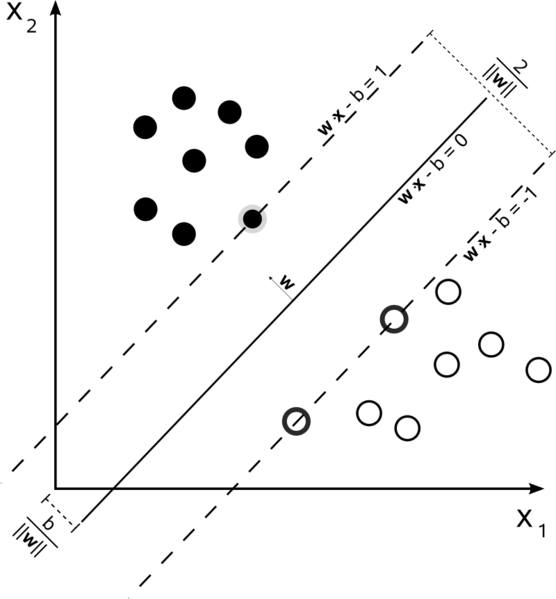
\includegraphics[width=0.5\textwidth]{Svm_max_sep_hyperplane_with_margin.png}
\caption{Margins for an SVM trained with samples from two classes}
\label{fig:svm_margin}
\end{figure}

This distance from the decision surface to the closest data point determines the margin of the classifier.

Therefore, the decision function for an \Acrshort{svm} is fully specified by a (usually small) subset of the data which defines the position of the separator, which can be seen in figure \ref{fig:svm_margin}. These points are referred to as the support vectors. They are called vectors because in a vector space, a point can be thought of as a vector between the origin and that point.


In ~\cite{Jagadanand2015}, a \Acrshort{svm} is used to classify stator fault in real time. To do so, the authors use \acrfull{cwt} to process the signal, then the wavelet coefficients of healthy and faulty motors are compared. After this, statistical parameters were found, like standard deviation, kurtosis and skewness, so that the relevant features for stator inter turn fault could be identified. The authors choose the standard deviation since it showed constant noticeable change in healthy and faulty condition of the motor. Then, the standard deviation was used to train the SVM.


In ~\cite{Patel2016}, a \Acrshort{svm} based scheme is used for condition monitoring and fault diagnosis of three-phase induction motor. Data of healthy motors and motors having faulty bearings, shorting of stator turns and broken rotor bars with varying load conditions was generated from laboratory. The scheme starts by calculating the total harmonic distortion of currents and voltages, thus forming feature vectors to train the \Acrshort{svm} classifier. This scheme provides an accuracy of more than 98\%.

The total harmonic distortion can be calculated as follows:

\begin{equation} 
\label{eq:total_harmornic_distortion}
THD_F = \frac{\sum_{i=2}^{n} V_i^2}{V_1}  
\end{equation}

\noindent where $V_n$ is the \acrshort{rms} value of the $nth$ harmonic and $n=1$ is th e fundamental frequency.

\subsection{Other approaches} % (fold)
\label{sec:other_approaches}


\acrfull{fl} is an approach of partitioning a feature space info fuzzy sets and utilizing fuzzy rules fore reasoning, which provides an approximate human reasoning ~\cite{Gao2015}. Several works have presented the successfully use of \acrshort{fl} for fault detection and diagnosis ~\cite{Azgomi2013, Zidani2008, JoverRodriguez2008}.
In  ~\cite{JoverRodriguez2008} the fuzzy system is based on knowledge expressed in rules and membership functions, describing the stator windings. The presented method has the hability to work with variable speed drives and is able to identify the motor stator condition with high accuracy.
In ~\cite{Xu-hong2007} the authors describe a fuzzy \acrshort{ann}  model trained using a genetic algorithm that provides a very flexible and specific response to nonlinear situations unique to a machine construction.

\acrfull{pso} is used in ~\cite{Liu2006}, where the author proposes this method to locale and determine the fault severity. \acrshort{pso} shares the ability of \acrshort{ann} and \acrfull{fl} systems to handle nonlinearities. This technique is train using both healthy motor data as well as faulty motor data, and starts with a random selection of particles and then iterates until the error is minimized.
 
\acrfull{cot} was applied in REF, where the technique is applied in order to improve the model in case of an unforeseen situation arises. This essentially allows the weighting of the \acrshort{ann} on a moving basis, and the model “forgets” previous weights. 